%TCIDATA{LaTeXparent=0,0,cap_RevisaoBibliografica.tex}

\section{Simulação Numérica de Reservatórios}

A simulação numérica de um reservatório é, segundo Peaceman, é o processo de inferência do comportamento do reservatório real dada a performance obtida de um modelo do mesmo, matemático ou físico (em escala laboratorial). Um modelo matemático de reservatório pode ser enxergado como um conjunto de equações diferenciais parciais, juntamente com as condições de contorno adequadas, que podem ser utilizadas para descrever satisfatoriamente os processos físicos importantes que ocorrem no sistema real.

Os processos que ocorrem em um reservatório são basicamente transporte de fluidos e transferência de massa; até três fases imiscíveis (óleo, gás e água) fluem simultaneamente, enquanto que o transporte de massa se dá entre as fases (notadamente entre o óleo e o gás). A gravidade, a capilaridade e as forças viscosas são também importantes no processo de vazão dos fluidos \cite{simres}.

Segundo Rosa, a primeira etapa de uma simulação numérica é formular o problema físico a ser representado matematicamente; em seguida são feitas suposições e simplificações compatíveis com o grau de sofisticação esperado do modelo, levando-se à formulação das equações matemáticas que descrevem o problema desejado, considerando-se as hipóteses adotadas. O passo seguinte é a resolução das equações e análise da solução obtida; posteriormente, a validade do simulador é verificada através da calibração com uma solução existente --- por exemplo, comparam-se os resultados obtidos do simulador numérico com soluções analíticas, resultados reais ou com resultados obtidos de modelos físicos de laboratório (dados experimentais). Caso o simulador seja considerado válido, o mesmo estará pronto para ser utilizado na simulação do fenômeno desejado; caso contrário, volta-se para um novo ciclo em que são revistas as hipóteses adotadas ou até a conceituação do modelo físico \cite[p. 520]{engres}. A Figura \ref{fig:rev_simuesq} esquematiza um desenvolvimento básico de um simulador numérico qualquer, enquanto que a Figura \ref{fig:rev_simuex} mostra uma comparação de resultados entre diferentes simuladores existentes, exemplificando o uso da calibração com soluções já obtidas para se validar um simulador de reservatório. 

\begin{figure}[!ht]
\centering
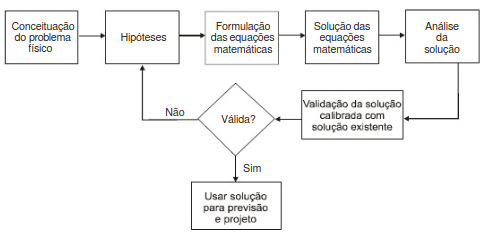
\includegraphics[width=.75\textwidth]{figs/revisao/revisao_simuesq.png}
\caption{Esquema básico de desenvolvimento de um simulador numérico de reservatório \cite[p. 519]{engres}.}\label{fig:rev_simuesq}
\end{figure}

\begin{figure}[!ht]
\centering
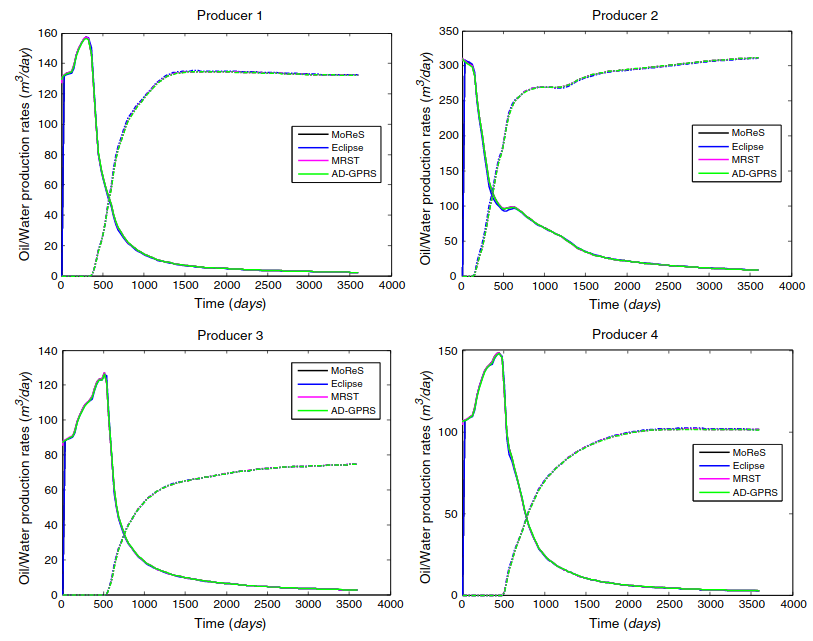
\includegraphics[width=.75\textwidth]{figs/revisao/revisao_simuex.png}
\caption{Exemplo de comparação de dados entre simuladores de vazão de água e de óleo de um modelo \cite{eggM}.}\label{fig:rev_simuex}
\end{figure}

\subsection{Leis Físicas Consideradas}

No caso de um simulador de reservatórios, as seguintes leis físicas básicas normalmente são consideradas, dependendo do tipo de simulador\footnote{Ver \cite[p. 520]{engres}}:

\begin{itemize}
\item Lei da conservação de massa;
\item Lei da conservação de energia;
\item Lei da conservação de \textit{``momentum''} (Segunda Lei de Newton):
\begin{equation}
\sum F = \frac{\partial M}{\partial t},
\end{equation}
onde $F$ representa uma força e $M = mv$ o \textit{``momentum''}, com $m$ sendo a massa e $v$ a velocidade.
\end{itemize}

Além das leis básicas da física, faz-se necessário o uso de várias leis, dependendo do simulador, que governam o comportamento dos fluidos envolvidos e a propriedade do reservatório estudado, apresentadas nas subseções a seguir\footnote{Os teoremas apresentados se encontram em \cite[pp. 520-522]{engres}}. Combinado-se as equações correspondentes às leis básicas, obtém-se uma equação diferencial parcial que rege o comportamento das variáveis dependentes em função das variáveis independentes e dos parâmetros do sistema. Como normalmente a equação obtida é não-linear, ela é, consequentemente, é resolvida por métodos númericos; daí a nomenclatura \textit{simulação numérica de reservatórios}.

\subsubsection{Fenômenos de Transporte}

\begin{theorem}[Lei de Darcy]
Na Lei de Darcy, ou lei do fluxo ``laminar'' ou Darcyano, a velocidade do fluxo viscoso de um fluido em meio poroso é dada por
\begin{equation}
	v_s = -\frac{k_s}{\mu} \frac{\partial\Phi}{\partial s},
\end{equation}
onde $k$ é a permeabilidade efetiva do meio ao fluido considerado, $\mu$ é a viscosidade do fluido, $\Phi$ é o potencial de fluxo e $s$ é a trajetória de fluxo.
\end{theorem}

\begin{theorem}[Lei de Forchheimer]
Também conhecida como lei do fluxo ``turbulento'' ou não-Darcyano, é utilizada para fluxos turbulentos, notadamente de gás; o gradiente de pressão é dado por
\begin{equation}
	-\frac{dp}{ds} = \frac{\mu}{k_s}v_s - \beta\rho v_s^2,
\end{equation}
onde $\rho$ é a massa específica do fluido e $\beta$ é o coeficiente de resistência inercial ou de fluxo não-Darcyano. 
\end{theorem}

\begin{theorem}[Lei de Fourier]
Durante um fenômeno de transporte de calor por condução, o fluxo de calor é dado por
\begin{equation}
	q_s = -k'\frac{\partial T}{\partial s},
\end{equation}
em que $k'$ é a condutividade térmica do meio e $T$ é a temperatura.
\end{theorem}

\begin{theorem}[Convecção]
O fluxo de calor no caso de tranporte por convecção é dado por
\begin{equation}
	q_s = c_p v_s (T - T_0),
\end{equation}
onde $c_p$ é a capacidade calorífica do fluido à pressão constante, $v$ a velocidade do fluido e $T_0$ uma temperatura de referência.
\end{theorem}

\subsubsection{Equações de Estado}
As principais equações de estado envolvidas na simulação do comportamento de um reservatório de petróleo são as que lidam com fluidos (líquidos ou gasosos) e rochas porosas. No caso de fluidos líquidos, tem-se a seguinte definição:

\begin{definition}
A compressibilidade isotérmica de um fluido é dada por
\begin{equation}
	c = -\frac{1}{V}\frac{\partial V}{\partial p} = \frac{1}{\rho}\frac{\partial \rho}{\partial p},
\end{equation}
em que $V$ é o volume, $p$ é a pressão e $\rho$ é a massa específica do fluido. Há algumas relações especiais para situações particulares:
\begin{itemize}
\item Líquidos de compressibilidade constante: $\rho = \rho_0 e^{c(p-p_0)}$.
\item Líquidos de compressibilidade constante e pequena: $\rho = \rho_0 \left[1+c\left(p-p_0\right)\right]$.
\end{itemize}
\end{definition}

Quando se trata de estudar o estado de um gás, se aplica a lei dos gases:
\begin{equation}\label{eq:gaslaw}
	\rho = \frac{pM}{ZRT}.
\end{equation}

A Equação \eqref{eq:gaslaw} pode ser aplicada tanto no caso de um gás real quanto de um gaś ideal; nela, $\rho$ é a massa específica do gás, $p$ é a pressão, $M$ é a massa molecular, $R$ é a constante universal dos gases, $T$ é a temperatura e $Z$ é o fator de compressibilidade do gás; no caso de um gás ideal, tem-se $Z = 1$.

Por fim, para se representar o comportamento da rocha, utiliza-se a equação da chamada compressibilidade efetiva:
\begin{equation}
	c_f = \frac{1}{\phi} \frac{\partial\phi}{\partial p},
\end{equation}
onde $c_f$ é a compressibilidade efetiva efetiva da formação e $\phi$, sua porosidade.

Além das leis até aqui citadas, cabe ressaltar que outras podem ser utilizadas em caso de simulações de fenômenos específicos, como injeção de vapor, injeção de polímeros, além de outros métodos empregados na produção de petróleo.

\subsection{Tipos de Simuladores}

\subsection{Uso de Simuladores Numéricos para Estudos de Reservatórios}